fgt\documentclass[12pt, %
openright, 
oneside, %
%twoside, %TCC: Se seu texto tem mais de 100 páginas, descomente esta linha e comente a anterior
a4paper,    %
%english,   %
brazil]{facom-ufu-abntex2}
\usepackage{xcolor}
% Definindo novas cores
\definecolor{verde}{rgb}{0.25,0.5,0.35}
\definecolor{jpurple}{rgb}{0.5,0,0.35}
% Configurando layout para mostrar codigos Java
\usepackage{listings}
\lstset{
  language=Java,
  basicstyle=\ttfamily\small, 
  keywordstyle=\color{jpurple}\bfseries,
  stringstyle=\color{red},
  commentstyle=\color{verde},
  morecomment=[s][\color{blue}]{/**}{*/},
  extendedchars=true, 
  showspaces=false, 
  showstringspaces=false, 
  numbers=left,
  numberstyle=\tiny,
  breaklines=true, 
  backgroundcolor=\color{cyan!10}, 
  breakautoindent=true, 
  captionpos=b,
  xleftmargin=0pt,
  tabsize=4
}
\autor{Patrick Godinho} %TCC
\data{2014}
\orientador{Lasaro Camargos} %TCC
%\coorientador{Algum?} %TCC 


% ---
% Informações de dados para CAPA e FOLHA DE ROSTO
% ---

\titulo{PheroCast App} %TCC

\hypersetup{pdfkeywords={palavra 1}{palavra 2}{palavra 4}{palavra 4}{palavra 5}} %TCC

\begin{document}
\frenchspacing 

% ----------------------------------------------------------
% ELEMENTOS PRÉ-TEXTUAIS
% ----------------------------------------------------------
%\pretextual
\imprimircapa
\imprimirfolhaderosto


% ---
% Inserir folha de aprovação
% ---
%
% \includepdf{folhadeaprovacao_final.png} %TCC: depois de aprovado o trabalho, descomente esta linha e comente o próximo bloco para incluir scan da folha de aprovação.
%
\begin{folhadeaprovacao}

  \begin{center}
    {\ABNTEXchapterfont\large\imprimirautor}

    \vspace*{\fill}\vspace*{\fill}
    {\ABNTEXchapterfont\bfseries\Large\imprimirtitulo}
    \vspace*{\fill}
    
    \hspace{.45\textwidth}
    \begin{minipage}{.5\textwidth}
        \imprimirpreambulo
    \end{minipage}%
    \vspace*{\fill}
   \end{center}
    
   Trabalho aprovado. \imprimirlocal, 24 de novembro de 2012: %TCC:

   \assinatura{\textbf{\imprimirorientador} \\ Orientador}  
   \assinatura{\textbf{Professor}}% \\ Convidado 1} %TCC:
   \assinatura{\textbf{Professor}}% \\ Convidado 2} %TCC:
   %\assinatura{\textbf{Professor} \\ Convidado 3}
   %\assinatura{\textbf{Professor} \\ Convidado 4}
      
   \begin{center}
    \vspace*{0.5cm}
    {\large\imprimirlocal}
    \par
    {\large\imprimirdata}
    \vspace*{1cm}
  \end{center}
  
\end{folhadeaprovacao}
% ---


%%As seções dedicatória, agradecimento e epígrafe não são obrigatórias.
%%Só as mantenha se achar pertinente.

% ---
% Dedicatória
% ---
\begin{dedicatoria}
   \vspace*{\fill}
   \centering
   \noindent
   \textit{Dedico a meu pai Paulo Sergio de Jesus Oliveira que sempre foi um exemplo de perseverança na minha vida!}  %TCC:
   \vspace*{\fill}
\end{dedicatoria}
% ---

% ---
% Agradecimentos
% ---
\begin{agradecimentos}
Agradeço a Deus, minha esposa e ao meu orientador Lasaro Camargos pelo apoio e dedicação para que eu conseguisse chegar ao final deste trabalho. %TCC:
\end{agradecimentos}
% ---

% ---
% Epígrafe
% ---
%\begin{epigrafe}
%    \vspace*{\fill}
%	\begin{flushright}
%		\textit{``Alguma citação que ache conveniente? \lipsum[10]''} %TCC:
%	\end{flushright}
%\end{epigrafe}
% ---



\begin{resumo} %TCC:

 \vspace{\onelineskip}
    
 \noindent
 \textbf{Palavras-chave}: Manet, Android, Redes Oportunísticas%TCC:
\end{resumo}

% ---
% inserir lista de ilustrações
% ---
\pdfbookmark[0]{\listfigurename}{lof}
\listoffigures*
\cleardoublepage
% ---

% ---
% inserir lista de tabelas
% ---
\pdfbookmark[0]{\listtablename}{lot}
\listoftables*
\cleardoublepage
% ---



% ---
% inserir lista de abreviaturas e siglas
% ---
%\begin{siglas} %TCC:
%  \item[Fig.] Area of the $i^{th}$ component
%  \item[456] Isto é um número
%  \item[123] Isto é outro número
%  \item[Zézão] este é o meu nome
%\end{siglas}
% ---

%% ---
%% inserir lista de símbolos, se for adequado ao trabalho. %TCC:
%% ---
%\begin{simbolos}
%  \item[$ \Gamma $] Letra grega Gama
%  \item[$ \Lambda $] Lambda
%  \item[$ \zeta $] Letra grega minúscula zeta
%  \item[$ \in $] Pertence
%\end{simbolos}
%% ---

% ---
% inserir o sumario
% ---
\pdfbookmark[0]{\contentsname}{toc}
\tableofcontents*
\cleardoublepage
% ---





% ----------------------------------------------------------
% ELEMENTOS TEXTUAIS
% ----------------------------------------------------------
\textual


% ----------------------------------------------------------
% Introdução
% ----------------------------------------------------------

\chapter{Introdução}
\addcontentsline{toc}{chapter}{Introdução}
%TCC:
\section{Contextualização}
\subsection{MANET}
MANET é a abreviação de Mobile Ad-Hoc Networks, a qual se define pelas redes em que nós se movimentam livremente, comunicam entre si e entre o meio em que está, sem a necessidade de nenhuma infraestrutura de rede. Tais ações permitem que várias aplicações sejam desenvolvidas com objetivo por exemplo da troca de informações entre os nós ou até o compartilhamento de serviços, como por exemplo a funcionalidade que temos hoje em dia de rotear a internet do celular com dispositivos próximos.

Também definida por \citetitle{de2002mobile} MANET pode ser conceituada como um sistema autonomo de servidores móveis (que tambem servem de roteadores), os quais unidos formam uma rede de comunicação representada por um grafo.

Os nós em uma MANET se movem arbitrariamente, e essa é a grande característica da rede, mas também o principal ofensor na qualidade da comunicação disponibilizada nesse ambiente, pois a arquitetura entre eles deve sempre estar se adaptando para os novos meios em que estão inseridos.

Desde que surgiu, a MANET tem sido vista como uma das mais desafiantes abordagens de redes móveis tanto pela promessa de crescimento de dispositivos móveis, quanto pela sua complexidade, o que impulsionou a pesquisa por esse paradigma. Apartir das pesqusias intensas na MANET, surgiram outras redes móveis baseadas em sua proposta inicial. Como por exemplo a VANET que será introduzida na próxima seção.

\subsection{VANET}
\subsubsection{Conceito}
VANET são redes móveis MANET onde os nós são os veículos e até a estrada, onde há comunicação apenas entre os automóveis (IVC - Inter Vehicle Communication), ou entre os mesmos e a estrada (RVC - Road Vehicle Communication).

Assim como na MANET, a Vehicular Ad-Hoc Network também permite que várias aplicações com vários objetivos sejam desenvolvidos, bem como alertar obstáculos na estrada, broadcast de informações de segurança, compartilhar informações de tráfego ou até solicitar socorro em algum acidente.

As simualções e experimentos tem tido um papel importante no desenvolvimento das soluções para redes veiculares. A atenção maior tem sido dada no desenvolvimento de modelos realistas de estrada e principalmente no estudo da mobilidade dos veículos. Por exemplo, modelos de como os carros se movem ao longo do trajeto, levando em consideração sua velocidade, sinais de transito, dentre outros fatores. 

\subsubsection{Problema}
O grande desafio das Redes Ad-Hoc Veiculares é o roteamento entre os nós, devida a alta taxa de mobilidade dos veículos que são conectados entre si intermitentemente, dificultando a entrega das mensagens entre os veículos ou estrada, pois frequentemente um nó muda seu endereço, ficando assim diferente de qual se identificou.

Além do problema citado acima, existe um agravante relacionado a velocidade de conexão entre os veículos, os quais se comunicam muito rápido, levando em consideração que os mesmos estejam em uma via rápida.

\subsection{Predição de localização}
\subsubsection{Motivo}
A predição da localidade de um nó, o qual pode ser um automóvel, uma pessoa com um dispositivo móvel, é algo bastante motivador a se desenvolver pelo fato de trazer otimizações da comunicação das redes MANET e suas derivadas, através da gestão proativa. \cite{6838650}

Por exemplo, caso um nó mande uma requisição para outro e logo após mude de localização, o responsável pela resposta será proativo o bastante para saber em qual posição o destinatário estará, resolvendo assim o problema da mobilidade, o qual é o principal desafio da VANET.

A predição de localização também é alvo de escopo de várias aplicações com o objetivo por exemplo de prever e otimizar tráfego em cidades inteligentes, ou até prever potenciais clientes para um passeio ecológico.

\subsubsection{PheroCast}
\paragraph{Conceito}
PheroCast é o nome que se deu à abordagem de previsão da localização futura de um nó em uma rede ad-hoc móvel. Foi nomeado assim pela semelhança com o fenomeno que acontece na colonia das formigas, o qual para alertar problemas, ou marcar o caminho, por onde a formiga passar, ela deixará um rastro, formando assim um caminho.

Nessa abordagem, o algoritmo de previsão é desenvolvido para ser processado nos próprios nós móveis. Assim, a cada intervalo de tempo definido, o nó registra um rastro de onde está. Daí vem a semelhança com o "Pheronomium" deixado no rastro por onde a formiga passa.

Assim, com o histórico dos "traces" de um determinado nó na forma de um grafo, é possível determinar uma probabilidade de onde ele estará em determinado horário apartir de um certo lugar.
\paragraph{Resultados}
Segundo \cite{6838650} foi feita uma avaliação do algoritmo PheroCast usando os caminhos dos onibus de Seattle Metro Transit, que vale a pena ressaltar, não foram extraídos para a abordagem nem com o intervalo de tempo ideal. Foi descoberto que a abordagem obteve bons resultados em relação à predição das futuras posicões dos onibus. A avaliação obteve 77,8\% de resultados positivos
\paragraph{Problema}
O grande problema do PheroCast é a sua avaliação limitada, ou seja, é necessário, para uma abordagem com essas características, uma avaliação extensa com dados reais, que ssimulam de verdade a mobilidade humana. 

Atualmente não existem "traces" reais, e sim módulos de mobilidade sintéticos, os quais não são realistas. Daí vem a proposta deste trabalho, o qual irá cooperar para avaliação confiável do PheroCast, coletando dados de mobilidade humana reais, através de seus dispositivos móveis.
\section{Proposta}
A proposta deste trabalho é desenvolver um sistema que rode em dispositivos móveis, para capturar "traces" reais de mobilidade humana. Para tal, o sistema irá coletar em um intervalo de tempo, todas as redes wireless, bem como suas informações, ao redor do dispositivo móvel do usuário e armazenar em um servidor para que os dados sejam compilados e utilizados para avaliação do PheroCast.

O objetivo é que o sistema seja utilizado por mais de um usuário para que assim tenhamos grande diversidade de histórico de traces.

\chapter{Referencial Teórico}
\section{PheroCast}
\section{Android}

\chapter{Proposta}
\section{Arquitetura}
A arquitetura proposta consiste em duas partes, clente e servidor. O cliente é responsável pela coleta dos dados, como posição atual, lista de SSID visíveis, e quaisquer outros dados que se deseje capturar. Oportunisticamente o cliente enviará os dados ao servidor. O servidor deverá consumir os dados enviados pelo dispositivo através de uma interface REST implementada e armazenar em um banco de dados, como mostra na Figura 1.  A seguir detalhamos cada um das partes.

\begin{figure}[hbt]
  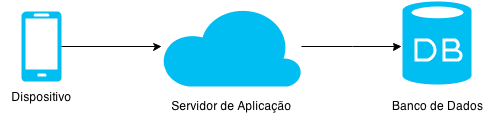
\includegraphics{arquiteturaProposta}
  \caption{Arquitetura Proposta}
\end{figure}


\subsection{Cliente}
Do lado do cliente desenvolveremos um sistema para rodar em dispositivos com o sistema operacional Android, utilizando a linguagem Java.

\begin{figure}[hbt]
  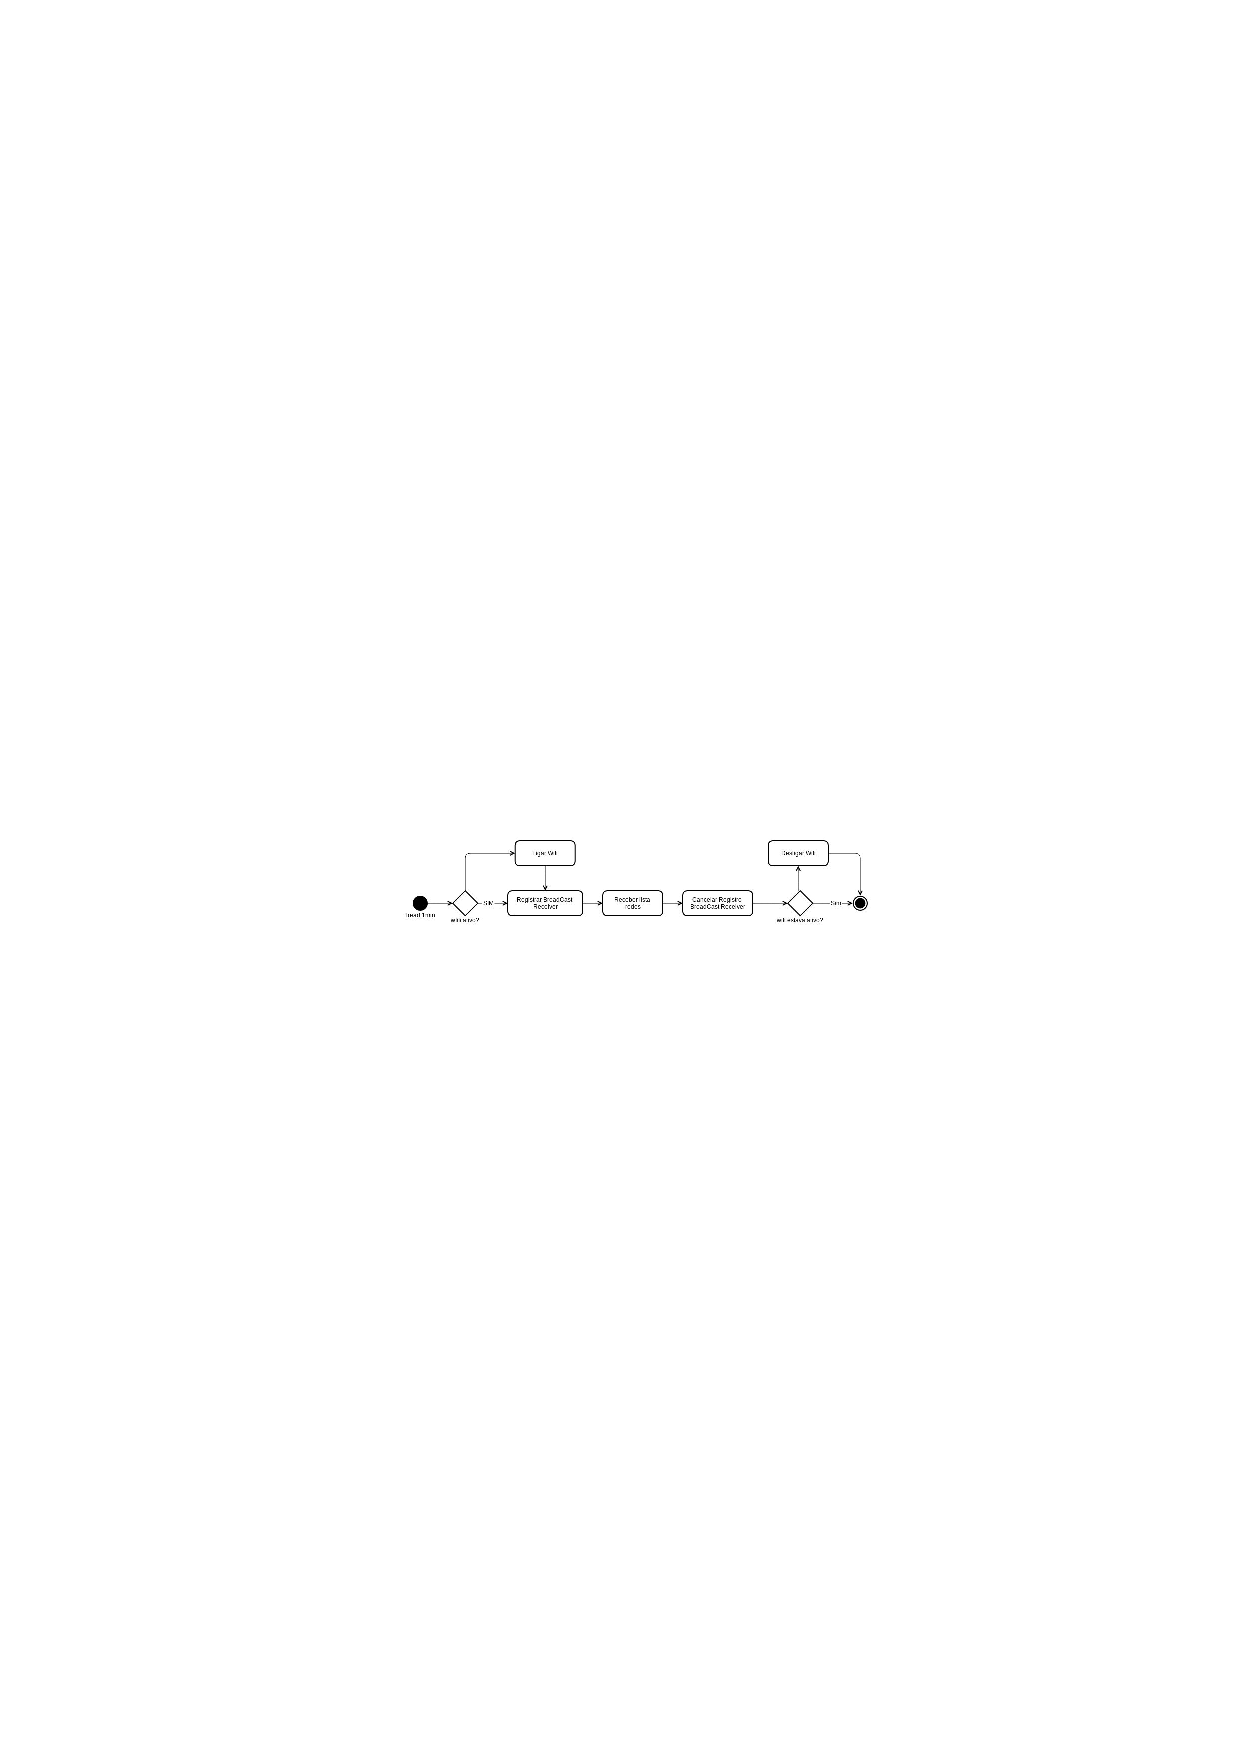
\includegraphics [scale=.4] {pherocast1}
  \caption{Processo de captura dos dados pelo aplicativo.}
\end{figure}

O aplicativo irá utilizar os serviços de Wifi do aparelho para realizar a coleta dos pontos de rede que estão ao redor naquele determinado momento. Após coleta, o sistema irá armazenar em base de dados local do dispositivo, para isso utilizaremos o banco de dados SQLite. Tal procedimento é ilustrado na Figura 2.

Para realizar o envio ao servidor, o aplicativo será alertado quando o dispositivo se conectar a uma rede WiFi com rede Internet, assim irá enviar os dados armazenados em sua base local para o servidor de aplicação na nuvem e apagar os mesmos. 

Caso o serviço de WiFi esteja desligado, o aplicativo deverá ser responsável por após ligar o Wifi e coletar os dados, desligar o mesmo, voltando assim para o estado inicial antes da coleta. Fazendo com que assim, não haja alteração no funcionamento do aparelho.




\subsection{Servidor}
Para o servidor, propomos utilizar algum servidor na nuvem de alta escalabilidade e alta disponibilidade, por se tratar de inserções contínuas todo o tempo.

O servidor deverá armazenar as informações virão do cliente, como:
\begin{itemize}
  \item SSID
  \item BSSID
  \item Recursos
  \item Frequencia
  \item Level
  \item Horário
  \item Identificador do Usuário do Dispositivo
  \end{itemize}
  
\subsection{Limpeza dos dados}
O sistema deverá tratar os dados do cliente com anonimidade, ou seja deverá haver algoritmos de segurança que tornem os dados do cliente anonimos, para preservar a identidade do usuário.
\chapter{Desenvolvimento}
\section{Aplicativo}
\section{Google Docs}
\section{Limpeza dos dados}

\chapter{Resultados}
\section{Dados Coletados}
\section{Análise}

\chapter{Conclusão}

%\chapter{Revisão Bibliográfica}
%TCC:

%Um ou mais capítulos (por exemplo, se há duas linhas de trabalhos relacionados.


% ----------------------------------------------------------
% ELEMENTOS PÓS-TEXTUAIS
% ----------------------------------------------------------
\postextual


% ----------------------------------------------------------
% Referências bibliográficas
% ----------------------------------------------------------
\bibliographystyle{plain}
\bibliography{bib}


%% ----------------------------------------------------------
%% Apêndices TCC: só mantenha se for pertinente.
%% ----------------------------------------------------------

% ---
% Inicia os apêndices
% ---


% ----------------------------------------------------------
% Anexos %TCC: so mantenha se pertinente.
% ----------------------------------------------------------

% ---
% Inicia os anexos
% ---
\begin{anexosenv}

% Imprime uma página indicando o início dos anexos
\partanexos

% ---
\chapter{Código fonte}
% 
\section{MainActivity.java}
\begin{lstlisting}
package ufu.tcc.patrick.pherocast;
import android.annotation.SuppressLint;
import android.content.BroadcastReceiver;
import android.content.Context;
import android.content.Intent;
import android.content.IntentFilter;
import android.net.wifi.ScanResult;
import android.net.wifi.WifiManager;
import android.os.Bundle;
import android.os.Handler;
import android.support.v7.app.ActionBarActivity;
import android.widget.TextView;
import android.widget.Toast;

import java.io.PrintStream;
import java.text.SimpleDateFormat;
import java.util.ArrayList;
import java.util.Date;
import java.util.List;
import java.util.Timer;
import java.util.TimerTask;

public class MainActivity extends ActionBarActivity {
	final Handler handler = new Handler();
	boolean scanInitiated;
	TimerTask scanTask;
	Timer t = new Timer();
	TextView text;
	WifiManager wifi;
	boolean wifiOn;
	WifiScanReceiver wifiReciever;
	String[] wifis;
	List<ScanResult> localList = new ArrayList<ScanResult>();

	private String pegarHoraAtual() {
		return new SimpleDateFormat("dd/MM/yyyy hh:mm:ss").format(new Date()); 
	}

	public void getWifiState() {
		System.out.println("passou aqui " + wifi.isWifiEnabled());
		if (!wifi.isWifiEnabled()) {
			wifiOn = false;
			Toast.makeText(getApplicationContext(),
					"Wifi desativado, estamos ativando...", 1).show();
			wifi.setWifiEnabled(true);
			return;
		}
		wifiOn = true;
	}

	public void onBackPressed() {
		moveTaskToBack(true);
	}

	protected void onCreate(Bundle paramBundle) {
		super.onCreate(paramBundle);
		setContentView(2130903064);
		wifi = ((WifiManager) getSystemService("wifi"));
		wifiReciever = new WifiScanReceiver();
		scanTask = new TimerTask() {
			public void run() {
				handler.post(new Runnable() {
					public void run() {
						getWifiState();
						registerReceiver(wifiReciever, new IntentFilter(
								"android.net.wifi.SCAN_RESULTS"));
						scanInitiated = true;
						wifi.startScan();
					}
				});
			}
		};
		t.schedule(scanTask, 300L, 60000L);
	}

	class WifiScanReceiver extends BroadcastReceiver {
		WifiScanReceiver() {
		}

		@SuppressLint({ "UseValueOf", "NewApi" })
		public void onReceive(Context paramContext, Intent paramIntent) {

			NetworkPointDAO localNetworkPointDAO = NetworkPointDAO
					.getInstance(getBaseContext());
			if (scanInitiated) {
				localList = wifi.getScanResults();
				wifis = new String[localList.size()];

			}
			for (int i = 0;; i++) {
				if (i >= localList.size()) {
					scanInitiated = false;
					System.out.println(wifiOn);
					if (!wifiOn)
						wifi.setWifiEnabled(false);
					unregisterReceiver(this);
					return;
				}
				wifis[i] = (((ScanResult) localList.get(i)).SSID + ", "
						+ ((ScanResult) localList.get(i)).frequency + ", "
						+ ((ScanResult) localList.get(i)).level + ", " + ((ScanResult) localList
						.get(i)).BSSID);
				localNetworkPointDAO
						.salvar(new NetworkPoint(
								((ScanResult) localList.get(i)).BSSID,
								((ScanResult) localList.get(i)).SSID,
								((ScanResult) localList.get(i)).capabilities,
								((ScanResult) localList.get(i)).frequency,
								((ScanResult) localList.get(i)).level,
								pegarHoraAtual()));
			}
		}
	}
}
\end{lstlisting}
\section{HttpRequest.java}
\begin{lstlisting}
package ufu.tcc.patrick.pherocast;


import java.io.IOException;
import java.io.InputStream;
import java.io.UnsupportedEncodingException;
import java.net.HttpURLConnection;
import java.net.URL;
import java.net.URLConnection;
import java.net.URLEncoder;

import org.apache.http.HttpResponse;
import org.apache.http.client.methods.HttpGet;
import org.apache.http.client.methods.HttpPost;
import org.apache.http.client.params.ClientPNames;
import org.apache.http.client.params.CookiePolicy;
import org.apache.http.entity.StringEntity;
import org.apache.http.impl.client.DefaultHttpClient;
import org.apache.http.params.BasicHttpParams;
import org.apache.http.params.HttpConnectionParams;
import org.apache.http.params.HttpParams;
import org.apache.http.protocol.BasicHttpContext;
import org.apache.http.protocol.HttpContext;
import org.apache.http.util.EntityUtils;
import org.json.JSONObject;

import android.util.Log;

/*
 * This helper class was created by StackOverflow user: MattC http://stackoverflow.com/users/21126/mattc
 * IT was posted as an Answer to this question: http://stackoverflow.com/questions/2253061/secure-http-post-in-android
 */

public class HttpRequest{

    DefaultHttpClient httpClient;
    HttpContext localContext;
    private String ret;

    HttpResponse response = null;
    HttpPost httpPost = null;
    HttpGet httpGet = null;

    public HttpRequest(){
        HttpParams myParams = new BasicHttpParams();

        HttpConnectionParams.setConnectionTimeout(myParams, 10000);
        HttpConnectionParams.setSoTimeout(myParams, 10000);
        httpClient = new DefaultHttpClient(myParams);       
        localContext = new BasicHttpContext();    
    }

    public void clearCookies() {
        httpClient.getCookieStore().clear();
    }

    public void abort() {
        try {
            if (httpClient != null) {
                System.out.println("Abort.");
                httpPost.abort();
            }
        } catch (Exception e) {
            System.out.println("Your App Name Here" + e);
        }
    }

    public String sendPost(String url, String data) {
        return sendPost(url, data, null);
    }

    public String sendJSONPost(String url, JSONObject data) {
        return sendPost(url, data.toString(), "application/json");
    }

    public String sendPost(String url, String data, String contentType) {
        ret = null;

        httpClient.getParams().setParameter(ClientPNames.COOKIE_POLICY, CookiePolicy.RFC_2109);

        httpPost = new HttpPost(url);
        response = null;

        StringEntity tmp = null;        

        Log.d("Your App Name Here", "Setting httpPost headers");

        httpPost.setHeader("User-Agent", "SET YOUR USER AGENT STRING HERE");
        httpPost.setHeader("Accept", "text/html,application/xml,application/xhtml+xml,text/html;q=0.9,text/plain;q=0.8,image/png,*;q=0.5");

        if (contentType != null) {
            httpPost.setHeader("Content-Type", contentType);
        } else {
            httpPost.setHeader("Content-Type", "application/x-www-form-urlencoded");
        }

        try {
            tmp = new StringEntity(data,"UTF-8");
        } catch (UnsupportedEncodingException e) {
            Log.e("Your App Name Here", "HttpUtils : UnsupportedEncodingException : "+e);
        }

        httpPost.setEntity(tmp);

        Log.d("Your App Name Here", url + "?" + data);

        try {
            response = httpClient.execute(httpPost,localContext);

            if (response != null) {
                ret = EntityUtils.toString(response.getEntity());
            }
        } catch (Exception e) {
            Log.e("Your App Name Here", "HttpUtils: " + e);
        }

        Log.d("Your App Name Here", "Returning value:" + ret);

        return ret;
    }

    public String sendGet(String url) {
        httpGet = new HttpGet(url);  

        try {
            response = httpClient.execute(httpGet);  
        } catch (Exception e) {
            Log.e("Your App Name Here", e.getMessage());
        }

        //int status = response.getStatusLine().getStatusCode();  

        // we assume that the response body contains the error message  
        try {
            ret = EntityUtils.toString(response.getEntity());  
        } catch (IOException e) {
            Log.e("Your App Name Here", e.getMessage());
        }

        return ret;
    }

    public InputStream getHttpStream(String urlString) throws IOException {
        InputStream in = null;
        int response = -1;

        URL url = new URL(urlString); 
        URLConnection conn = url.openConnection();

        if (!(conn instanceof HttpURLConnection))                     
            throw new IOException("Not an HTTP connection");

        try{
            HttpURLConnection httpConn = (HttpURLConnection) conn;
            httpConn.setAllowUserInteraction(false);
            httpConn.setInstanceFollowRedirects(true);
            httpConn.setRequestMethod("GET");
            httpConn.connect(); 

            response = httpConn.getResponseCode();                 

            if (response == HttpURLConnection.HTTP_OK) {
                in = httpConn.getInputStream();                                 
            }                     
        } catch (Exception e) {
            throw new IOException("Error connecting");            
        } // end try-catch

        return in;     
    }
    

	public void postData() {
		String fullUrl = "https://docs.google.com/forms/d/1AYvV0gFgB1hBuoRKnMsXy1LyF8-Ce8VAshAtho6Z08s/formResponse";
		HttpRequest mReq = new HttpRequest();
		String col1 = "Hello";
		String col2 = "World";

		String data = "entry.1680144410=" + URLEncoder.encode(col1) + "&" + 
					  "entry.1558298396=" + URLEncoder.encode(col2);
		String response = mReq.sendPost(fullUrl, data);
		Log.i("DocsUpload", response);
	} 
}

\end{lstlisting}
\section{NetworkChangeReceiver.java}
\begin{lstlisting}
package ufu.tcc.patrick.pherocast;

import android.content.BroadcastReceiver;
import android.content.Context;
import android.content.Intent;
import android.net.ConnectivityManager;
import android.net.NetworkInfo;
import android.util.Log;
import java.io.PrintStream;
import java.net.URLEncoder;
import java.util.ArrayList;
import java.util.Iterator;

public class NetworkChangeReceiver extends BroadcastReceiver
{
  public void enviarParaDocs(Context paramContext)
  {
    NetworkPointDAO localNetworkPointDAO = NetworkPointDAO.getInstance(paramContext);
    ArrayList localArrayList = (ArrayList)localNetworkPointDAO.recuperarTodos();
    HttpRequest localHttpRequest = new HttpRequest();
    Iterator localIterator = localArrayList.iterator();
    while (true)
    {
      if (!localIterator.hasNext())
        return;
      NetworkPoint localNetworkPoint = (NetworkPoint)localIterator.next();
      String str1 = localNetworkPoint.getSsid();
      String str2 = localNetworkPoint.getBssid();
      String str3 = localNetworkPoint.getCapabilities();
      String str4 = String.valueOf(localNetworkPoint.getFrequency());
      String str5 = String.valueOf(localNetworkPoint.getLevel());
      String str6 = localNetworkPoint.getData();
      String str7 = UserEmailFetcher.getEmail(paramContext);
      localHttpRequest.sendPost("https://docs.google.com/forms/d/1G_dkyvwug--i_We7qAaA3QV-Xw_plTBJeKdElW22S4w/formResponse", "entry_2059700=" + URLEncoder.encode(str1) + "&" + "entry_1828317397=" + URLEncoder.encode(str2) + "&" + "entry_2146852893=" + URLEncoder.encode(str3) + "&" + "entry_312023197=" + URLEncoder.encode(str4) + "&" + "entry_644637792=" + URLEncoder.encode(str5) + "&" + "entry_604910793=" + URLEncoder.encode(str6) + "&" + "entry_612999935= " + URLEncoder.encode(str7));
      localNetworkPointDAO.deletar(localNetworkPoint);
    }
  }

  public void onReceive(final Context paramContext, Intent paramIntent)
  {
    ConnectivityManager localConnectivityManager = (ConnectivityManager)paramContext.getSystemService("connectivity");
    NetworkInfo localNetworkInfo1 = localConnectivityManager.getNetworkInfo(1);
    NetworkInfo localNetworkInfo2 = localConnectivityManager.getNetworkInfo(0);
    if ((localNetworkInfo1.isAvailable()) || (localNetworkInfo2.isConnected()));
    try
    {
      new Thread(new Runnable()
      {
        public void run()
        {
          enviarParaDocs(paramContext);
        }
      }).start();
      return;
    }
    catch (Exception localException)
    {
      Log.d("Netowk Available ", localException.getMessage());
    }
  }
}

\end{lstlisting}
\section{NetworkPoint.java}
\begin{lstlisting}
package ufu.tcc.patrick.pherocast;

public class NetworkPoint
{
  private String bssid;
  private String capabilities;
  private String data;
  private int frequency;
  private int level;
  private String ssid;
  private long timestamp;

  public NetworkPoint()
  {
  }

  public NetworkPoint(String paramString1, String paramString2, String paramString3, int paramInt1, int paramInt2, String paramString4)
  {
    this.bssid = paramString1;
    this.ssid = paramString2;
    this.capabilities = paramString3;
    this.frequency = paramInt1;
    this.level = paramInt2;
    this.data = paramString4;
  }

  public String getBssid()
  {
    return this.bssid;
  }

  public String getCapabilities()
  {
    return this.capabilities;
  }

  public String getData()
  {
    return this.data;
  }

  public int getFrequency()
  {
    return this.frequency;
  }

  public int getLevel()
  {
    return this.level;
  }

  public String getSsid()
  {
    return this.ssid;
  }

  public long getTimestamp()
  {
    return this.timestamp;
  }

  public void setBssid(String paramString)
  {
    this.bssid = paramString;
  }

  public void setCapabilities(String paramString)
  {
    this.capabilities = paramString;
  }

  public void setData(String paramString)
  {
    this.data = paramString;
  }

  public void setFrequency(int paramInt)
  {
    this.frequency = paramInt;
  }

  public void setLevel(int paramInt)
  {
    this.level = paramInt;
  }

  public void setSsid(String paramString)
  {
    this.ssid = paramString;
  }

  public void setTimestamp(long paramLong)
  {
    this.timestamp = paramLong;
  }
}

\end{lstlisting}
\section{NetworkPointDAO.java}
\begin{lstlisting}
package ufu.tcc.patrick.pherocast;

import android.content.ContentValues;
import android.content.Context;
import android.database.Cursor;
import android.database.sqlite.SQLiteDatabase;
import java.io.PrintStream;
import java.util.ArrayList;
import java.util.List;

public class NetworkPointDAO
{
  public static final String COLUNA_BSSID = "bssid";
  public static final String COLUNA_CAPABILITIES = "capabilities";
  public static final String COLUNA_DATA = "data_adicao";
  public static final String COLUNA_FREQUENCIA = "frequencia";
  public static final String COLUNA_LEVEL = "level";
  public static final String COLUNA_SSID = "ssid";
  public static final String COLUNA_TIMESTAMP = "timestamp";
  public static final String NOME_TABELA = "network_point";
  public static final String SCRIPT_CRIACAO_TABELA_NETWORK_POINT = "CREATE TABLE network_point(bssid TEXT, ssid TEXT, capabilities TEXT, frequencia INTEGER, level INTEGER, timestamp LONG, data_adicao STRING )";
  public static final String SCRIPT_DELECAO_TABELA = "DROP TABLE IF EXISTS network_point";
  private static NetworkPointDAO instance;
  private SQLiteDatabase dataBase = null;

  private NetworkPointDAO(Context paramContext)
  {
    this.dataBase = PersistenceHelper.getInstance(paramContext).getWritableDatabase();
  }

  private List<NetworkPoint> construirNetworkPorCursor(Cursor paramCursor)
  {
    ArrayList localArrayList = new ArrayList();
    if (paramCursor == null)
      return localArrayList;
    try
    {
      if (paramCursor.moveToFirst())
      {
        boolean bool;
        do
        {
          int i = paramCursor.getColumnIndex("ssid");
          int j = paramCursor.getColumnIndex("bssid");
          int k = paramCursor.getColumnIndex("capabilities");
          int m = paramCursor.getColumnIndex("frequencia");
          int n = paramCursor.getColumnIndex("level");
          paramCursor.getColumnIndex("timestamp");
          int i1 = paramCursor.getColumnIndex("data_adicao");
          String str1 = paramCursor.getString(i);
          String str2 = paramCursor.getString(j);
          String str3 = paramCursor.getString(k);
          int i2 = paramCursor.getInt(n);
          localArrayList.add(new NetworkPoint(str2, str1, str3, paramCursor.getInt(m), i2, paramCursor.getString(i1)));
          bool = paramCursor.moveToNext();
        }
        while (bool);
      }
      return localArrayList;
    }
    finally
    {
      paramCursor.close();
    }
    //throw localObject;
  }

  private ContentValues gerarContentValues(NetworkPoint paramNetworkPoint)
  {
    ContentValues localContentValues = new ContentValues();
    localContentValues.put("bssid", paramNetworkPoint.getBssid());
    localContentValues.put("ssid", paramNetworkPoint.getSsid());
    localContentValues.put("capabilities", paramNetworkPoint.getCapabilities());
    localContentValues.put("frequencia", Integer.valueOf(paramNetworkPoint.getFrequency()));
    localContentValues.put("level", Integer.valueOf(paramNetworkPoint.getLevel()));
    localContentValues.put("data_adicao", paramNetworkPoint.getData());
    return localContentValues;
  }

  public static NetworkPointDAO getInstance(Context paramContext)
  {
    if (instance == null)
      instance = new NetworkPointDAO(paramContext);
    return instance;
  }

  public void deletar(NetworkPoint paramNetworkPoint)
  {
    String[] arrayOfString = new String[1];
    arrayOfString[0] = String.valueOf(paramNetworkPoint.getBssid());
    this.dataBase.delete("network_point", "bssid =  ?", arrayOfString);
  }

  public void editar(NetworkPoint paramNetworkPoint)
  {
    ContentValues localContentValues = gerarContentValues(paramNetworkPoint);
    String[] arrayOfString = new String[1];
    arrayOfString[0] = String.valueOf(paramNetworkPoint.getBssid());
    this.dataBase.update("network_point", localContentValues, "bssid = ?", arrayOfString);
  }

  public void fecharConexao()
  {
    if ((this.dataBase != null) && (this.dataBase.isOpen()))
      this.dataBase.close();
  }

  public int getQuantidade()
  {
    return this.dataBase.rawQuery("select * from network_point", null).getCount();
  }

  public List<NetworkPoint> recuperarTodos()
  {
    return construirNetworkPorCursor(this.dataBase.rawQuery("SELECT * FROM network_point", null));
  }

  public void salvar(NetworkPoint paramNetworkPoint)
  {
    ContentValues localContentValues = gerarContentValues(paramNetworkPoint);
    this.dataBase.insert("network_point", null, localContentValues);
    System.out.println(paramNetworkPoint.getData() + "AUHUHAHUU");
  }

  public void truncarTabela()
  {
    this.dataBase.execSQL("DELETE FROM network_point;");
  }
}
\end{lstlisting}
\section{PersistenceHelper.java}
\begin{lstlisting}
package ufu.tcc.patrick.pherocast;

import android.content.Context;
import android.database.sqlite.SQLiteDatabase;
import android.database.sqlite.SQLiteOpenHelper;

public class PersistenceHelper extends SQLiteOpenHelper
{
  public static final String NOME_BANCO = "wificollector";
  public static final int VERSAO = 1;
  private static PersistenceHelper instance;

  private PersistenceHelper(Context paramContext)
  {
    super(paramContext, "wificollector", null, 1);
  }

  public static PersistenceHelper getInstance(Context paramContext)
  {
    if (instance == null)
      instance = new PersistenceHelper(paramContext);
    return instance;
  }

  public void onCreate(SQLiteDatabase paramSQLiteDatabase)
  {
    paramSQLiteDatabase.execSQL("CREATE TABLE network_point(bssid TEXT, ssid TEXT, capabilities TEXT, frequencia INTEGER, level INTEGER, timestamp LONG, data_adicao STRING )");
  }

  public void onUpgrade(SQLiteDatabase paramSQLiteDatabase, int paramInt1, int paramInt2)
  {
    paramSQLiteDatabase.execSQL("DROP TABLE IF EXISTS network_point");
    onCreate(paramSQLiteDatabase);
  }
}

\end{lstlisting}
\section{UserEmailFetcher.java}
\begin{lstlisting}
package ufu.tcc.patrick.pherocast;

import android.accounts.Account;
import android.accounts.AccountManager;
import android.content.Context;
import android.util.Log;

public class UserEmailFetcher
{
  private static Account getAccount(AccountManager paramAccountManager)
  {
    Account[] arrayOfAccount = paramAccountManager.getAccountsByType("com.google");
    if (arrayOfAccount.length > 0)
      return arrayOfAccount[0];
    return null;
  }

  static String getEmail(Context paramContext)
  {
    Account localAccount = getAccount(AccountManager.get(paramContext));
    if (localAccount == null)
      return null;
    Log.w("TESTE DE EMAIL", localAccount.name);
    return localAccount.name;
  }
}

\end{lstlisting}

\end{anexosenv}

%---------------------------------------------------------------------
% INDICE REMISSIVO
%---------------------------------------------------------------------

\printindex

\end{document}
